\documentclass{beamer}

\usepackage{graphicx}
\usepackage[sfdefault,light]{FiraSans}
%\usefonttheme{serif} 
\usepackage[british]{datetime2}
\usetheme{default}
\setbeamertemplate{navigation symbols}{} % No navigation symbols
\setbeamercolor{alerted text}{fg=blue!80!green!159!}
\setbeamercolor{frame title}{fg=blue!80!green!159!}
\setbeamercolor{title}{fg=blue!80!green!159!}
\setbeamercolor{subtitle}{fg=blue!80!green!159!}

\makeatletter
\setbeamertemplate{footline}
{
  \leavevmode%
  \hbox{%
  \begin{beamercolorbox}[wd=.15\paperwidth,ht=2.25ex,dp=1ex,center]{institute in head/foot}%
    \usebeamerfont{title in head/foot}%
    \raisebox{-0.15cm}{
\includegraphics[width=1cm]{logo_ntnu_u-slagord.pdf}}
  \end{beamercolorbox}%
  \begin{beamercolorbox}[wd=.6\paperwidth,ht=2.25ex,dp=1ex,center]{institute in head/foot}%
    \usebeamerfont{title in head/foot}%
    \insertsection
  \end{beamercolorbox}%
  \begin{beamercolorbox}[wd=.15\paperwidth,ht=2.25ex,dp=1ex,center]{institute in head/foot}%
    \usebeamerfont{title in head/foot}%
    \insertshortdate
  \end{beamercolorbox}%
  \begin{beamercolorbox}[wd=.1\paperwidth,ht=2.25ex,dp=1ex,right]{institute in head/foot}%
    \usebeamerfont{title in head/foot} 
    \insertframenumber{} / \inserttotalframenumber\hspace*{2ex} 
  \end{beamercolorbox}}%
}
\makeatother

%----------------------------------------------------------------------------------------
%	TITLE PAGE
%----------------------------------------------------------------------------------------

\title{POL2012: Theories and Models in Political Economy}
\subtitle{Neo-Classical Political Economy}
% \date{\today}
\date{}
\author{Marius Swane Wishman}
\institute{Department of Sociology and Political Science}

\begin{document}

\begin{frame}[plain]
\titlepage % Print the title page as the first slide
\centering % Comment out if second logo

\includegraphics[width=5cm]{logo_ntnu_u-slagord.pdf}
%\hspace{0.5cm} 
\includegraphics[width=5cm]{logo_ntnu_u-slagord.pdf} % Second logo
\end{frame}


\section{Neo-classical political economy} % Sections can be created in order to organize your presentation into discrete blocks, all sections and subsections are automatically printed in the table of contents as an overview of the talk
%------------------------------------------------


\begin{frame}{Historical Context - A Crisis of Capitalism}

	\begin{figure}
		\centering
		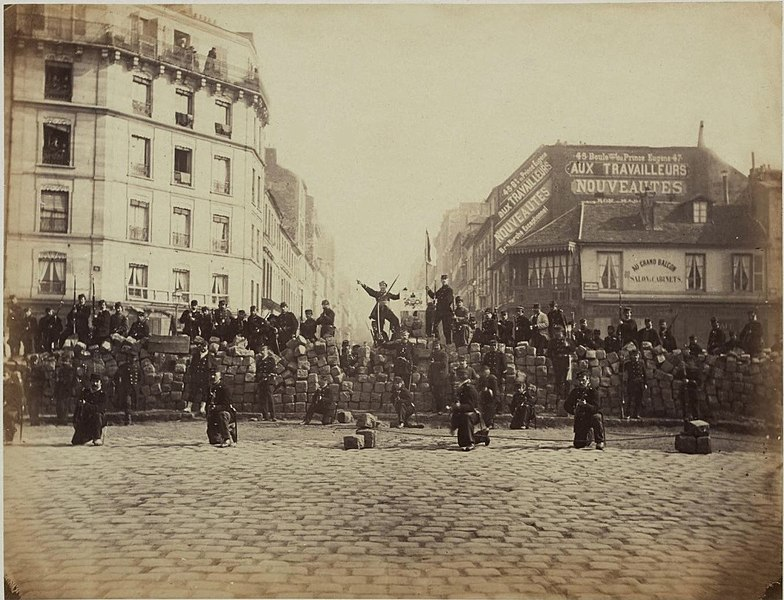
\includegraphics[width=0.8\linewidth]{../img/Commune.jpg}
		\label{commune}
	\end{figure}

\end{frame}

\begin{frame}{Historical Context - A Crisis of Capitalism}

	\begin{figure}[]
		\centering
		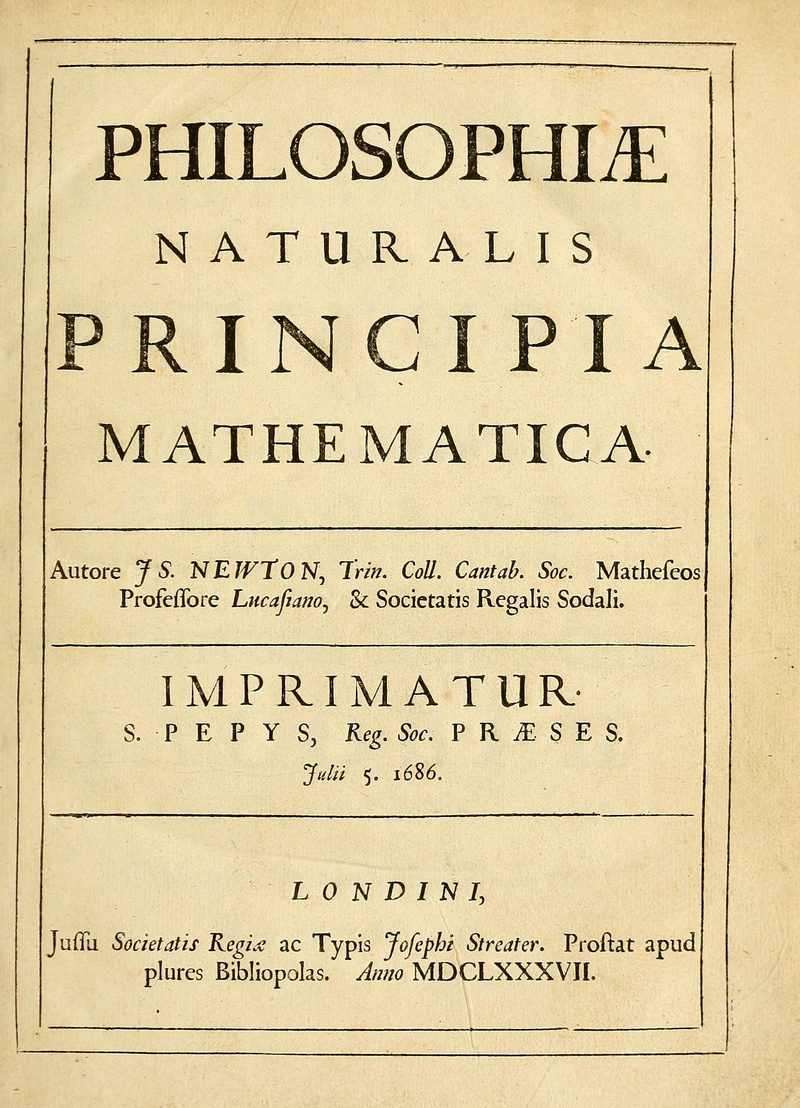
\includegraphics[width=0.8\linewidth]{../img/Prinicipia.png}
		\label{Principia}
	\end{figure}

\end{frame}


\begin{frame}{Supply and Demand}

	\begin{figure}[htpb]
		\centering
		\includegraphics[width=0.8\linewidth]{../img/supply-and-demand.png}
	\end{figure}

\end{frame}{}

\begin{frame}{Supply and Demand}

\begin{columns}[onlytextwidth]

	\column{.33\textwidth}
	\begin{figure}[htpb]
		\centering
		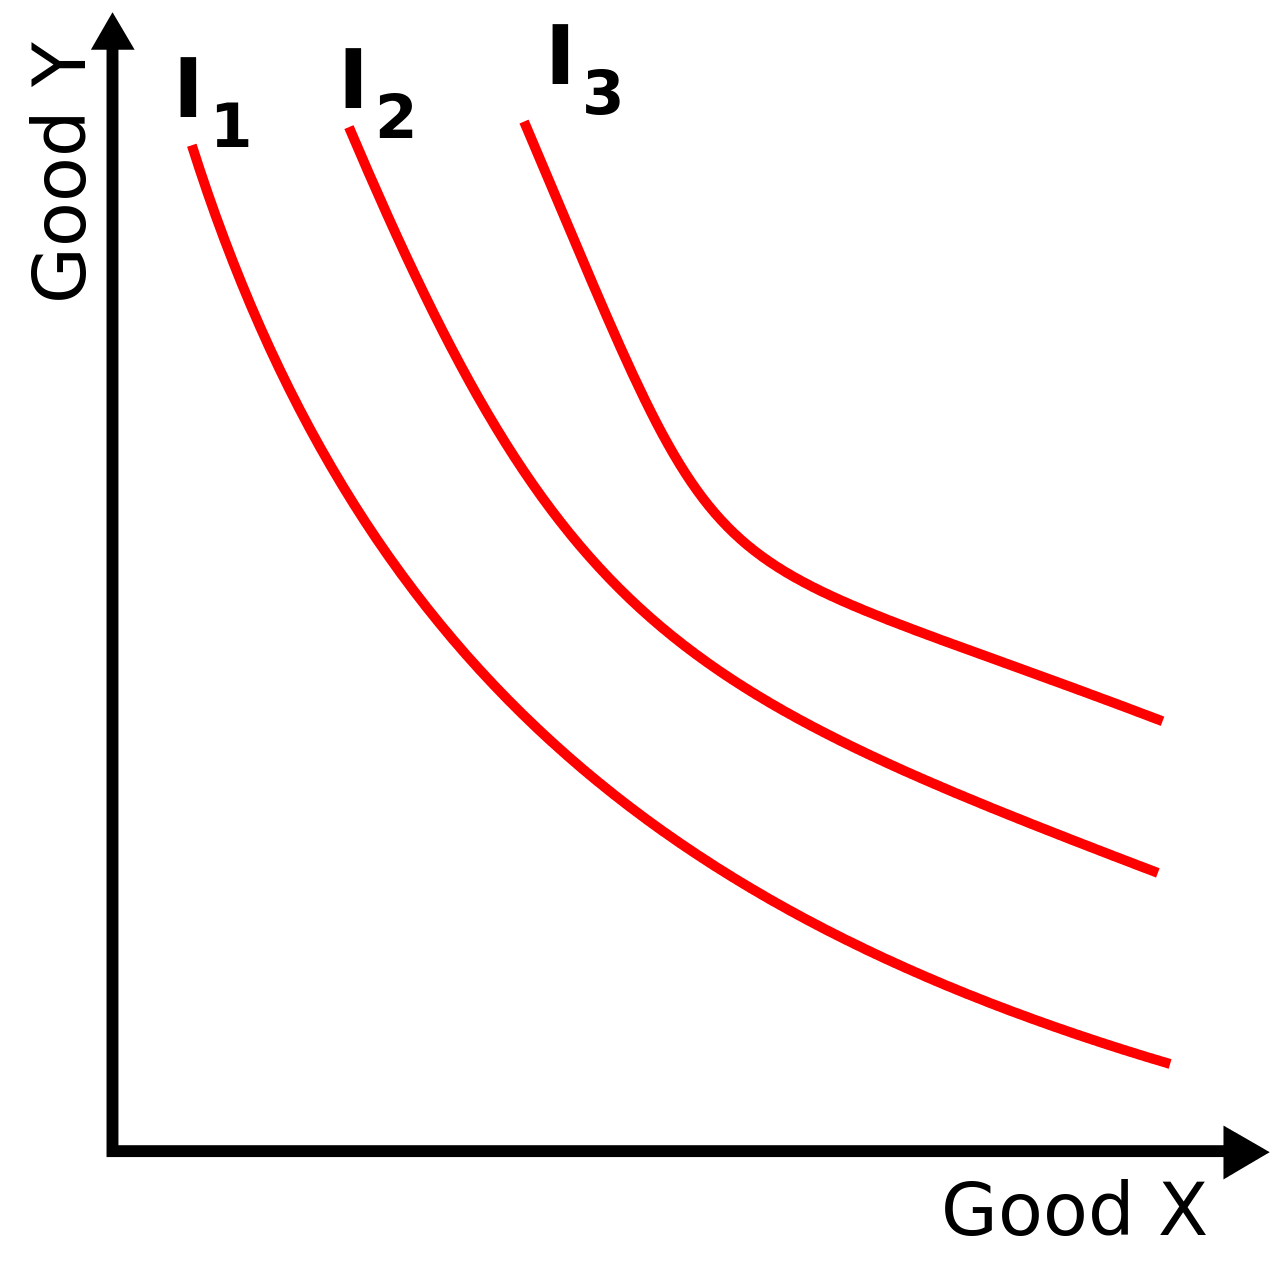
\includegraphics[width=0.8\linewidth]{../img/indifferent1.png}
		\caption{An example of an indifference map with three
		indifference curves represented}
		\label{fig:indif1}
	\end{figure}

	\column{.33\textwidth}
	\begin{figure}[htpb]
		\centering
		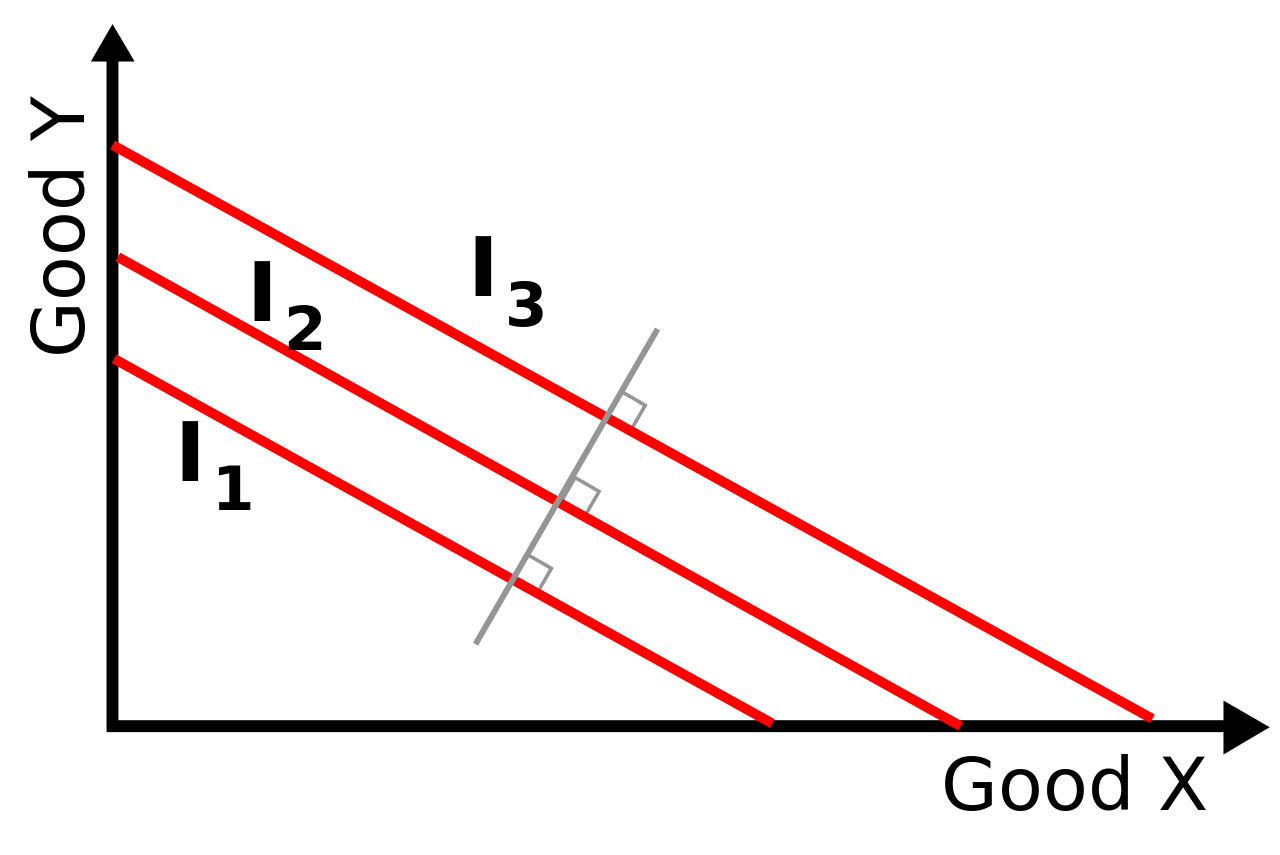
\includegraphics[width=0.8\linewidth]{../img/indifferent2.png}
		\caption{Three indifference curves where Goods X and Y are
			perfect substitutes.}
		\label{fig:indif2}
	\end{figure}

		\column{.33\textwidth}
	\begin{figure}[htpb]
		\centering
		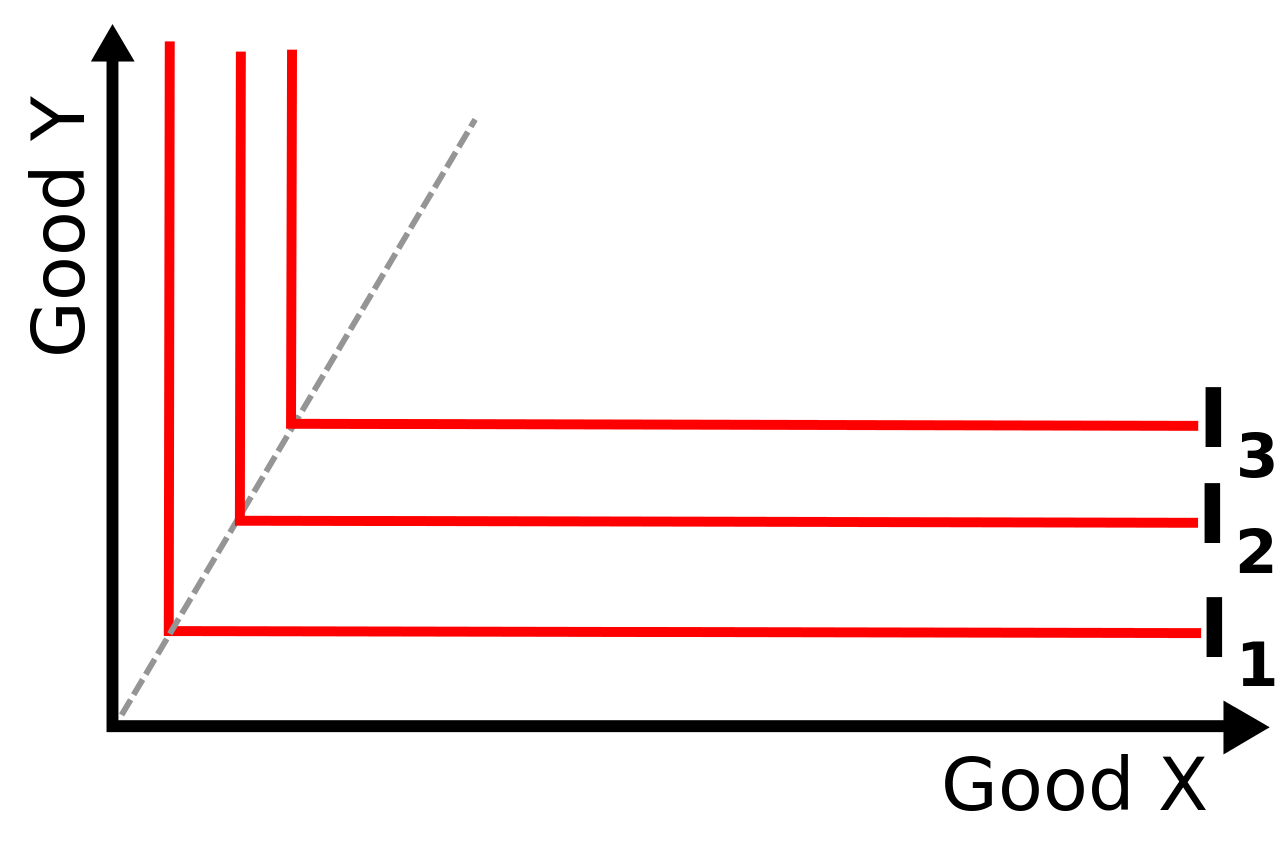
\includegraphics[width=0.8\linewidth]{../img/indifferent3.png}
		\caption{Indifference curves for perfect complements X and Y.}
		\label{fig:indif3}
	\end{figure}

\end{columns}
\end{frame}

\begin{frame}{Assumptions}
    \begin{itemize}[<+- | alert@+>]
    \item Utility % Explains differences and maximization % Value, Smith
    \item Rational actors
    \item Information and competition
    %\item Class, competing interests?
    \end{itemize}
\end{frame}{}

\begin{frame}{Benefits}
\end{frame}

\begin{frame}{Benefits}
	\begin{figure}[htpb]
		\centering
		
\includegraphics[width=0.8\linewidth]{../img/science.jpeg}
	\end{figure}
\end{frame}

\begin{frame}{Benefits}
	\begin{figure}[htpb]
		\centering
		
\includegraphics[width=0.6\linewidth]{../img/prediction.png}
	\end{figure}
\end{frame}

\begin{frame}{Units of analysis}

	\begin{columns}[onlytextwidth]
		\column{.5\textwidth}

		\begin{figure}[htpb]
			\centering
			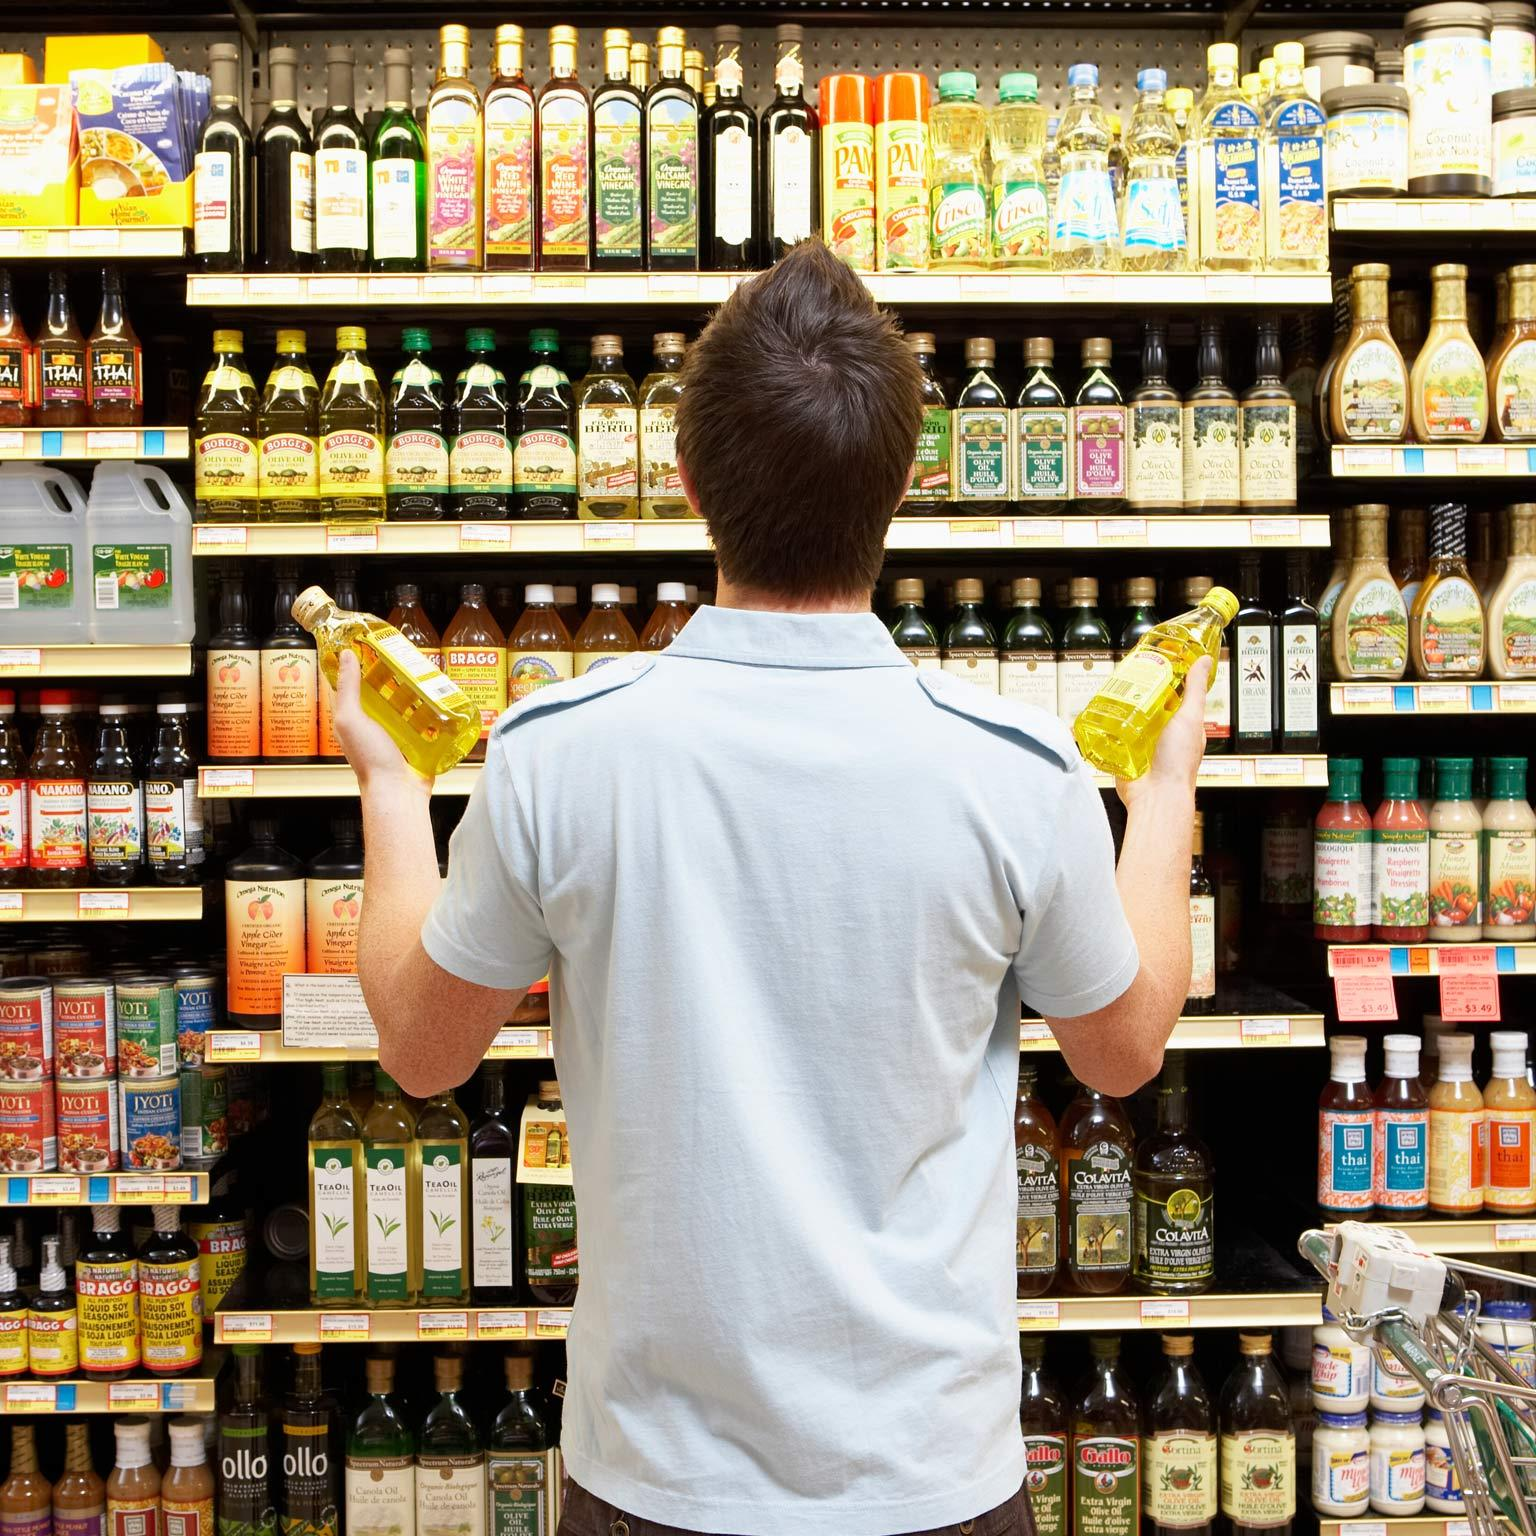
\includegraphics[width=0.8\linewidth]{../img/consumer.jpeg}
		\end{figure}

		\column{.5\textwidth}

		\begin{figure}[htpb]
			\centering
			
\includegraphics[width=0.8\linewidth]{../img/firms.jpg}
		\end{figure}
	\end{columns}

\end{frame}{}

\begin{frame}{The paradox of the firm}

	\begin{figure}[htpb]
		\centering
		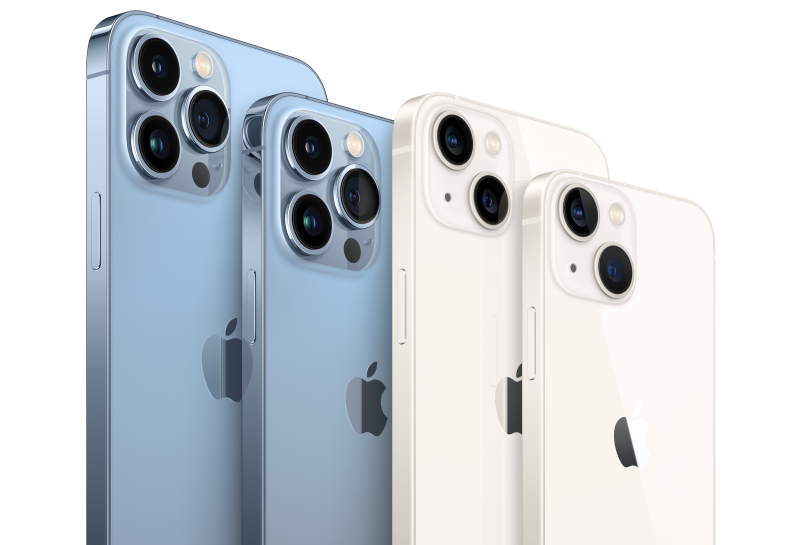
\includegraphics[width=0.8\linewidth]{../img/iphone.png}
	\end{figure}

\end{frame}

\begin{frame}{How should we structure the market?}
\end{frame}

\begin{frame}{How should we structure the market?}
    \begin{itemize}
    \item Perfect competition
    \end{itemize}
\end{frame}{}

\begin{frame}{Distribution}
	\begin{figure}[htpb]
		\centering
		
\includegraphics[width=0.8\linewidth]{../img/dontdoit.jpeg}
	\end{figure}
\end{frame}{}

\begin{frame}{Summary discussions}
\end{frame}

\end{document} 
